\documentclass[unknownkeysallowed]{beamer}

\usepackage[utf8]{inputenc}
\usepackage{graphicx}
\usepackage{epsfig}
\usepackage{hyperref}
\usepackage{booktabs, caption}
\usepackage{color}
\usepackage{tikz}


\beamertemplatenavigationsymbolsempty

\mode<presentation>
{
  \usetheme{sebslides}
  \setbeamertemplate{items}[circle]
}

\definecolor{uipoppy}{RGB}{225, 64, 5}
\definecolor{tumblue}{RGB}{0,100,188}
\definecolor{uipaleblue}{RGB}{96,123,139}
\definecolor{uiblack}{RGB}{0, 0, 0}

\newcommand{\topline}{%
  \tikz[remember picture,overlay] {%
    \draw[line width=0.35mm, uipaleblue]
    ([yshift=-1.2cm]current page.north west)
    -- ([yshift=-1.2cm,xshift=\paperwidth]current page.north west);}}

\title{Data Mining with Spare Grids}
\subtitle{Seminar: Computational Aspects of Machine Learning}
\author{Sebastian Kreisel}
\date{\today}


\begin{document}

{
\setbeamertemplate{footline}{}
\begin{frame}
  \maketitle
  \vspace{15px}
  \begin{center}
    \color{tumblue}{\footnotesize{Technische Universität München}}\\
    \vspace{6px}
    \includegraphics[width=1cm]{tum}
  \end{center}
\end{frame}
}
\addtocounter{framenumber}{-1}

\begin{frame}
  \frametitle{Overview}
  \topline
  \vspace{-10px}
  \begin{itemize}
    \item Motivation for Sparse Grids
      \vspace{8px}
    \item Sparse Grids: Basics
      \vspace{8px}
    \item Sparse Grids: Machine Learning
      \vspace{8px}
    \item Examples with Data Sets
      \vspace{8px}
    \item Parallelization and Implementation
  \end{itemize}
\end{frame}

\begin{frame}
  \frametitle{Motivation for Sparse Grids}
  \topline
  \vspace{-10px}
  \begin{block}{Grid based approaches in ML}
    \begin{itemize}
      \item Discretizes the space into a grid
      \item Basis--functions around grid points, not data points
    \end{itemize}

    \begin{figure}[!htb]
      \setbeamertemplate{caption}{\raggedright\insertcaption\par}
      \setbeamerfont{caption}{size=\footnotesize}
      \minipage{0.45\textwidth}
      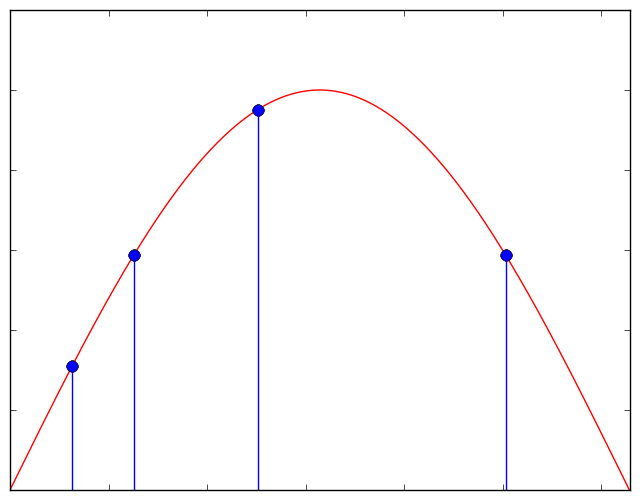
\includegraphics[width=\linewidth]{images/pointbase.png}
      \vspace{-12px}
      \caption{Point based}
      \endminipage
      \hspace{0.025\textwidth}
      \minipage{0.45\textwidth}
      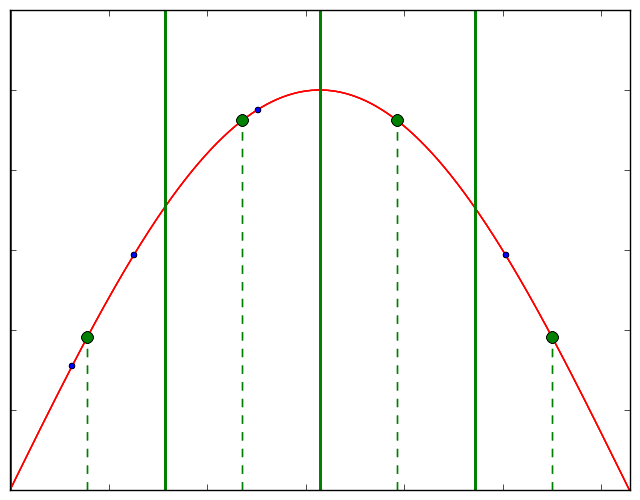
\includegraphics[width=\linewidth]{images/gridbase.png}
      \vspace{-12px}
      \caption{Grid based}
      \endminipage
    \end{figure}
  \end{block}
\end{frame}

\begin{frame}
  \frametitle{Motivation for Sparse Grids}
  \topline
  \vspace{-10px}
  \begin{block}{Suitable for}
    \begin{itemize}
      \item Big datasets
      \item Easily/automatically classifiable data
      \item Medical, seismic, commercial data
    \end{itemize}
  \end{block}
  \begin{block}{Curse of dimensionality}
    \begin{itemize}
    \item The volume of a space is exponential in it's dimensions
    \item The amount of training data required becomes unmanageable
      \begin{itemize}
      \item because of lacking computational/storage capacities
      \item because data acquisition is expensive
      \end{itemize}
    \item Becomes relevant for $d > 3$
    \item \textbf{Applies to full-grid discretization}
    \end{itemize}
  \end{block}
\end{frame}

%%% Local Variables:
%%% TeX-master: "slides"
%%% End:
\begin{frame}
  \frametitle{Full Grid Discretization}
  \topline1
  \vspace{-10px}
  \begin{block}{1. Function to discretize}
    \begin{figure}[!htp]

      \setbeamertemplate{caption}{\raggedright\insertcaption\par}
      \setbeamerfont{caption}{size=\footnotesize}
      \centering
      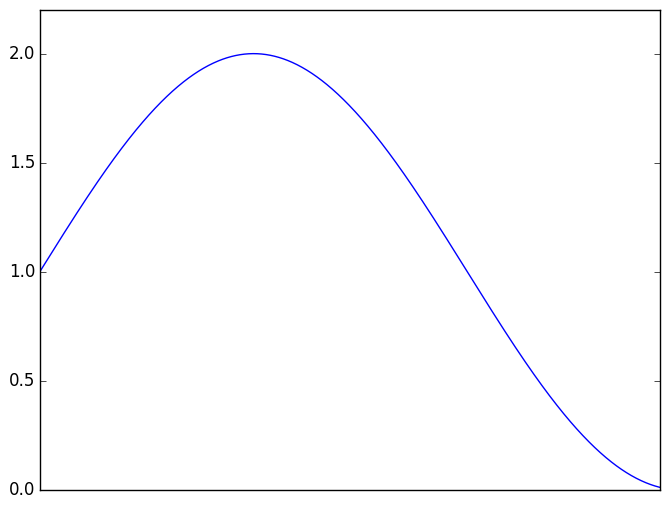
\includegraphics[width=7.5cm]{images/singlebasis_1}
      \vspace{-12px}
      \caption{$f(x) =\text{sin}(2\pi \cdot x)$}
    \end{figure}
  \end{block}
\end{frame}

\begin{frame}
  \frametitle{Full Grid Discretization}
  \topline
  \vspace{-10px}
  \begin{block}{2. Full, regular grid}
    \begin{figure}[!htp]

      \setbeamertemplate{caption}{\raggedright\insertcaption\par}
      \setbeamerfont{caption}{size=\footnotesize}
      \centering
      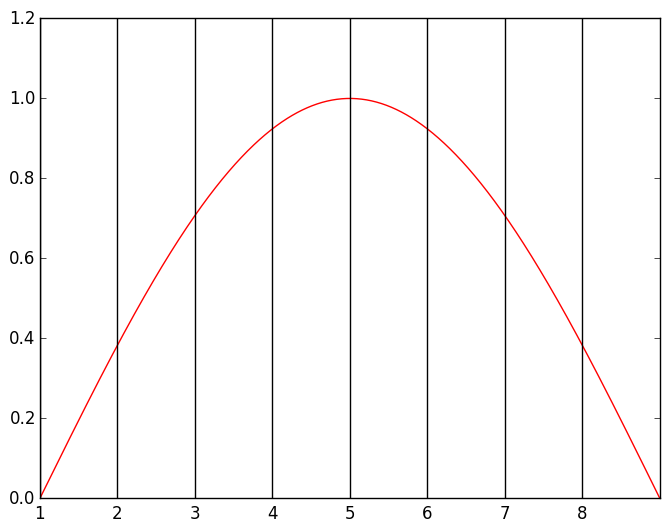
\includegraphics[width=7.5cm]{images/singlebasis_2}
      \vspace{-12px}
      \caption{7 grid points $i \in \{1..7\}$}
    \end{figure}
  \end{block}
\end{frame}

\begin{frame}
  \frametitle{Full Grid Discretization}
  \topline
  \vspace{-10px}
  \begin{block}{3. Basis function (standard hat function)}
    \begin{figure}[!htp]

      \setbeamertemplate{caption}{\raggedright\insertcaption\par}
      \setbeamerfont{caption}{size=\footnotesize}
      \centering
      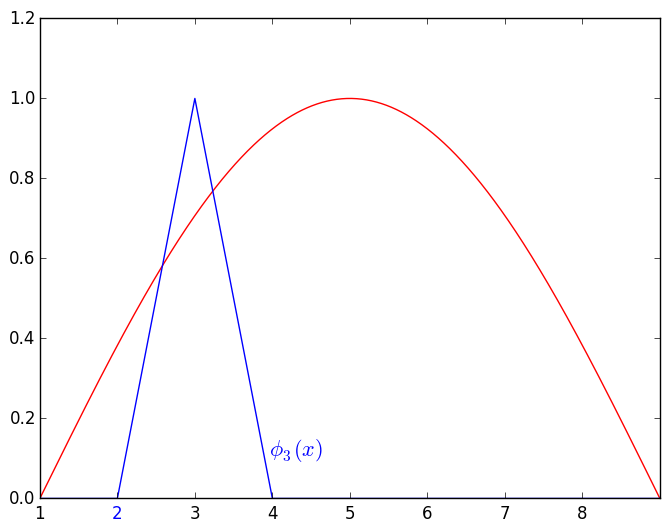
\includegraphics[width=7.5cm]{images/singlebasis_3}
      \vspace{-12px}
      \caption{$\phi(x - 3)$ with $\phi(x) = \text{max}(|1 - x|, 0)$}
    \end{figure}
  \end{block}
\end{frame}

\begin{frame}
  \frametitle{Full Grid Discretization}
  \topline
  \vspace{-10px}
  \begin{block}{4. Coefficient $\alpha$ (Surplus)}
    \begin{figure}[!htp]

      \setbeamertemplate{caption}{\raggedright\insertcaption\par}
      \setbeamerfont{caption}{size=\footnotesize}
      \centering
      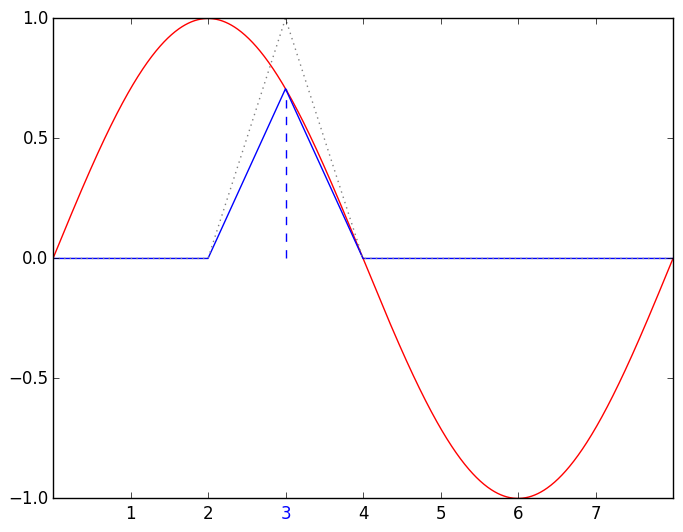
\includegraphics[width=7.5cm]{images/singlebasis_4}
      \vspace{-12px}
      \caption{$\alpha_3 \cdot \phi_3(x)$}
    \end{figure}
  \end{block}
\end{frame}

\begin{frame}
  \frametitle{Full Grid Discretization}
  \topline
  \vspace{-10px}
  \begin{block}{Sum over all basis functions}
    \begin{figure}[!htp]

      \setbeamertemplate{caption}{\raggedright\insertcaption\par}
      \setbeamerfont{caption}{size=\footnotesize}
      \centering
      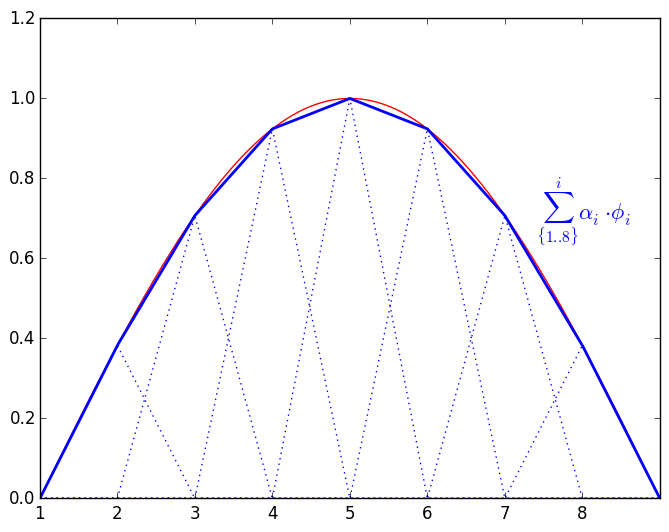
\includegraphics[width=7.5cm]{images/singlebasis_5}
      \vspace{-12px}
      \caption{$f(x) \approx \hat{f}(x) = \sum_i{\alpha_i \phi_i}$}
    \end{figure}
  \end{block}
\end{frame}

\begin{frame}
  \frametitle{Full Grid Discretization}
  \topline
  \vspace{-10px}
  \begin{block}{Sum over all basis functions}
    \begin{figure}[!htp]

      \setbeamertemplate{caption}{\raggedright\insertcaption\par}
      \setbeamerfont{caption}{size=\footnotesize}
      \centering
      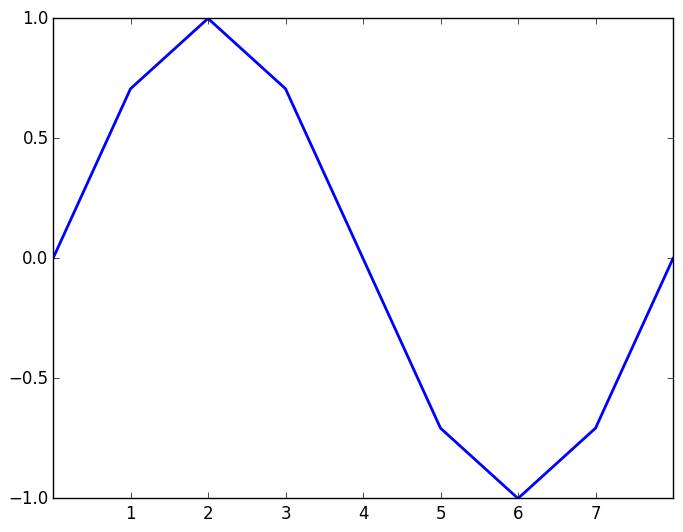
\includegraphics[width=7.5cm]{images/singlebasis_6}
      \vspace{-12px}
      \caption{$f(x) \approx \hat{f}(x) = \sum_i{\alpha_i \phi_i}$}
    \end{figure}
  \end{block}
\end{frame}

\begin{frame}
  \frametitle{Full Grid Discretization}
  \topline
  \vspace{-10px}
  \begin{block}{Full grid discretization in one dimension}
    \setbeamertemplate{enumerate items}[default]
    \begin{enumerate}
    \item A function $f(x)$ to discretize
    \item Grid points indexed by $i \in \{1,2,\dots\}$
    \item Basis functions; i.e. hat function $\phi(x)=\text{max}(1 - |x|, 0)$
    \item Coefficients $\alpha_i$ (Surpluses)
    \end{enumerate}
    \vspace{10px}
    \begin{center}
      $f(x) \approx$ $\hat{f}(x) = \sum_{i}^{}{\alpha_i \phi_i(x)}$
    \end{center}
  \end{block}
\end{frame}

\begin{frame}
  \frametitle{Full Grid Discretization}
  \topline
  \vspace{-10px}
  \begin{block}{$d > 1$ dimensions}
    \begin{itemize}
      \item Grid points as $d$--tuple, i.e. $(1,3,1)$
      \item Tensor product over one dimensional basis functions
    \end{itemize}
    \begin{center}
      $$ \phi_i(\vec{x}) = \prod_{j=1}^d{\phi_{i,j}(x_j)}$$
      $$ f(\vec{x}) \approx \hat{f}(\vec{x}) =
      \sum_i{\alpha_i\phi_i(\vec{x})}$$
    \end{center}
  \end{block}
\end{frame}

\begin{frame}
  \frametitle{Full Grid Discretization}
  \topline
  \vspace{-10px}
  \begin{block}{Full grid with $d = 2$}

    \begin{figure}[!htb]
      \setbeamertemplate{caption}{\raggedright\insertcaption\par}
      \setbeamerfont{caption}{size=\footnotesize}
      \minipage{0.5\textwidth}
      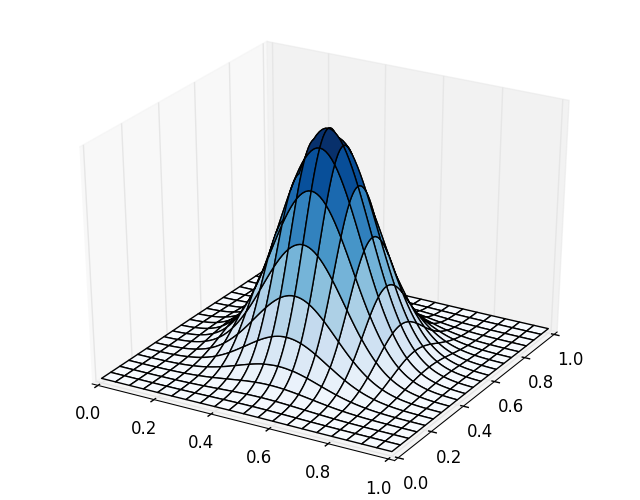
\includegraphics[width=\linewidth]{images/2dgrid_1_1.png}
      \vspace{-12px}
      \caption{$f(x) = \mathcal{N}(\vec{x})$}
      \endminipage
      \minipage{0.5\textwidth}
      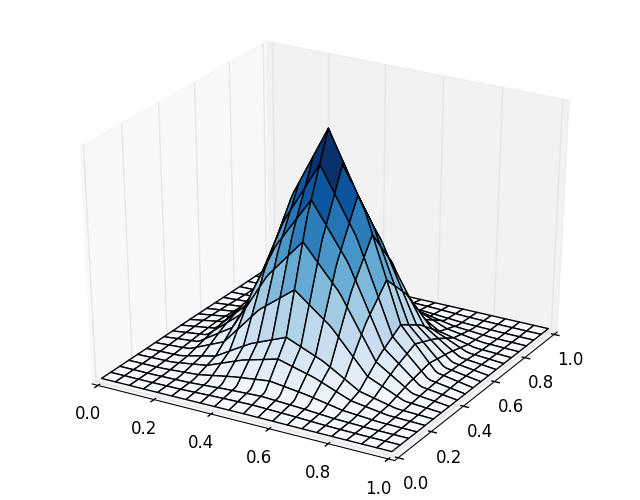
\includegraphics[width=\linewidth]{images/2dgrid_2_1.png}
      \vspace{-12px}
      \caption{Full grid discretization $\hat{f}(\vec{x})$}
      \endminipage
    \end{figure}
  \end{block}
\end{frame}

\begin{frame}
  \frametitle{Full Grid Discretization}
  \topline
  \vspace{-10px}
  \begin{block}{Full grid with $d = 2$}

    \begin{figure}[!htb]
      \setbeamertemplate{caption}{\raggedright\insertcaption\par}
      \setbeamerfont{caption}{size=\footnotesize}
      \minipage{0.5\textwidth}
      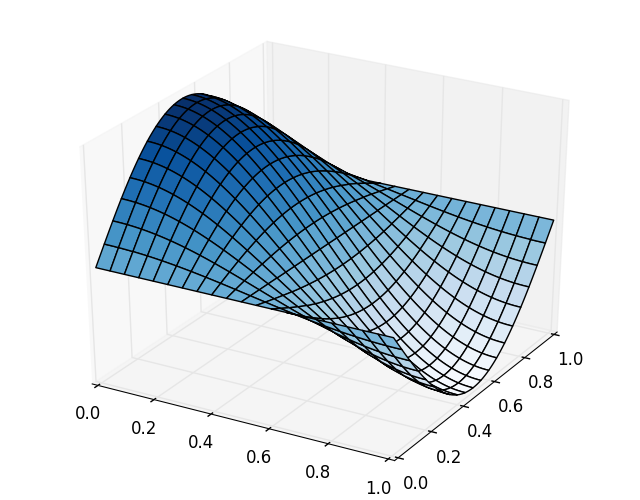
\includegraphics[width=\linewidth]{images/2dgrid_1_2.png}
      \vspace{-12px}
      \caption{$f(x) = \text{sin}(x_1) \cdot \text{cos}(x_2)$}
      \endminipage
      \minipage{0.5\textwidth}
      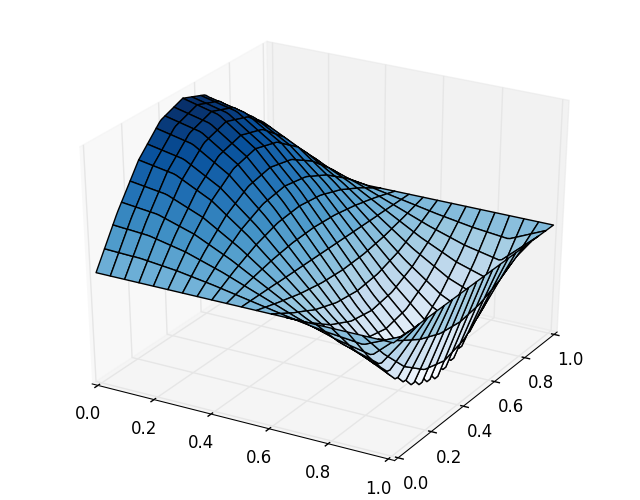
\includegraphics[width=\linewidth]{images/2dgrid_2_2.png}
      \vspace{-12px}
      \caption{Full grid discretization $\hat{f}(\vec{x})$}
      \endminipage
    \end{figure}
  \end{block}
\end{frame}

\begin{frame}
  \frametitle{Full Grid Discretization}
  \topline
  \vspace{-10px}
  \begin{block}{Summary}
    \begin{itemize}
      \item Grid points $i \in \{1,2,\dots,N\}^d$ defining $\phi_i(x)$
        \vspace{5px}
        \item For $d > 1$: \textbf{product} of 1D basis functions: \\
          $$\phi_i(\vec{x}) = \prod_{j=1}^d{\phi_{i,j}(x_j)}$$
        \item \textbf{Sum} over all weighted basis functions: \\
          $$\hat{f}(\vec{x}) = \sum_{i=1}^N{\alpha_i \phi_i(\vec{x})}$$
    \end{itemize}

  \end{block}
\end{frame}

%%% Local Variables:
%%% TeX-master: "slides"
%%% End:

\begin{frame}
  \frametitle{Sparse Grids -- Basics}
  \topline
  \vspace{-10px}
  \begin{block}{Hirachial Basis}
    \begin{figure}[!htp]
      \setbeamertemplate{caption}{\raggedright\insertcaption\par}
      \setbeamerfont{caption}{size=\footnotesize}
      \centering
      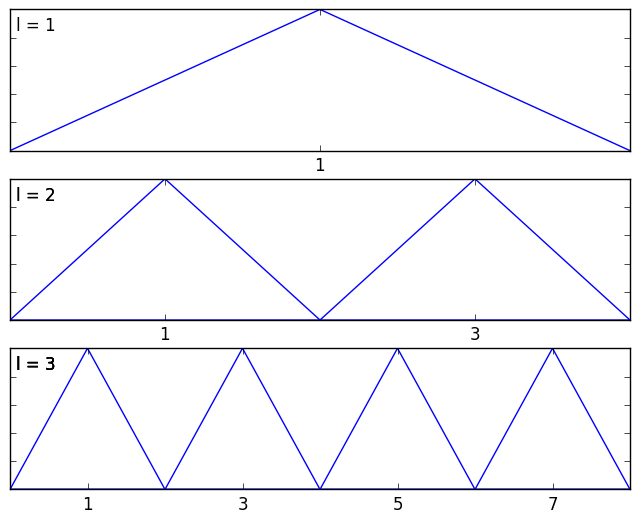
\includegraphics[width=7.5cm]{images/sparse_hats}
      \vspace{-12px}
      \caption{}
    \end{figure}
  \end{block}
\end{frame}

\begin{frame}
  \frametitle{Sparse Grids -- Basics}
  \topline
  \vspace{-10px}
  \begin{block}{Hirachial basis (vs nodal basis)}
    \begin{itemize}
      \item Grouping gridpoints into levels $l \in \{1,2,3\dots\}$
      \item Basis function by index \textbf{and} level: $\phi_{l,i}(x)$
    \end{itemize}
    \vspace{20px}
    \begin{center}
      $\hat{f}(x) = \sum_{l,i}{\ \alpha_{l,i} \cdot \phi_{l,i}(x)}$
    \end{center}
  \end{block}
\end{frame}

\begin{frame}
  \frametitle{Sparse Grids -- Basics}
  \topline
  \vspace{-10px}
  \begin{block}{Hirachial Basis}
    \begin{figure}[!htp]
      \setbeamertemplate{caption}{\raggedright\insertcaption\par}
      \setbeamerfont{caption}{size=\footnotesize}
      \centering
      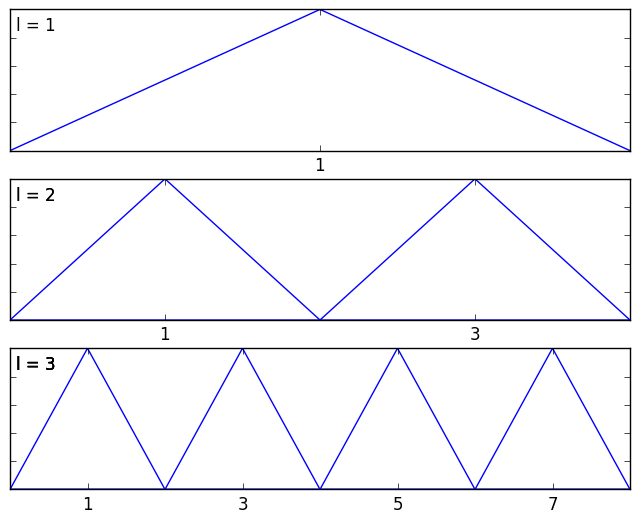
\includegraphics[width=7.5cm]{images/sparse_hats}
      \vspace{-12px}
      \caption{}
    \end{figure}
  \end{block}
\end{frame}

\begin{frame}
  \frametitle{Sparse Grids -- Basics}
  \topline
  \vspace{-10px}
  \begin{block}{Hirachial vs. nodal  basis}
    \begin{figure}[!htp]
      \setbeamertemplate{caption}{\raggedright\insertcaption\par}
      \setbeamerfont{caption}{size=\footnotesize}
      \centering
      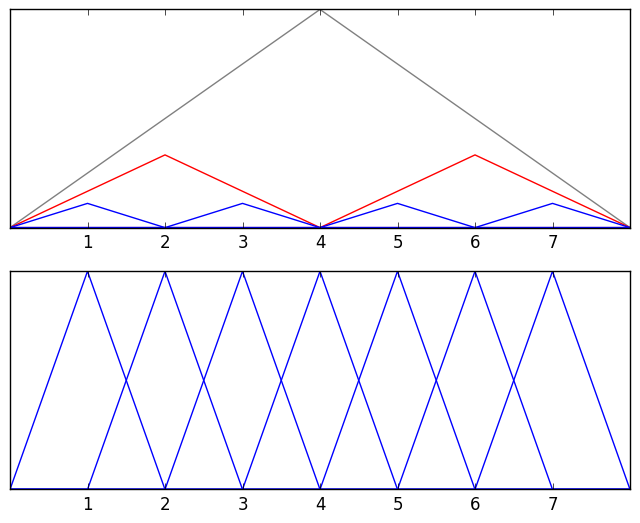
\includegraphics[width=7.5cm]{images/sparse_together}
      \vspace{-12px}
      \caption{}
    \end{figure}
  \end{block}
\end{frame}

\begin{frame}
  \frametitle{Sparse Grids -- Basics}
  \topline
  \vspace{-10px}
  \begin{block}{Full grid discretization: Hirachial basis}
    \begin{figure}[!htp]
      \setbeamertemplate{caption}{\raggedright\insertcaption\par}
      \setbeamerfont{caption}{size=\footnotesize}
      \centering
      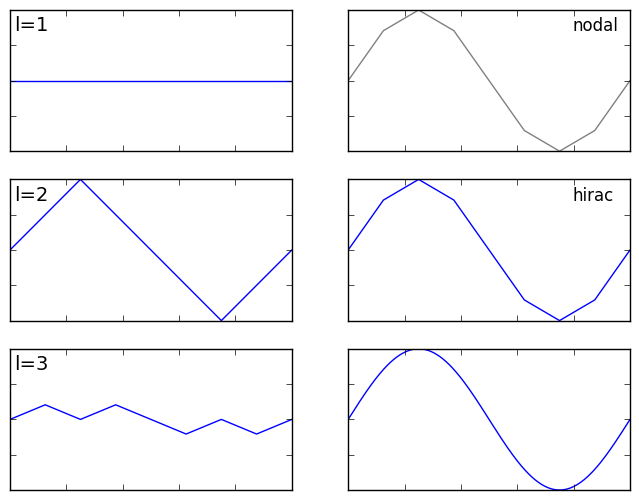
\includegraphics[width=7.5cm]{images/sparsegrid_1d}
      \vspace{-12px}
      \caption{}
    \end{figure}
  \end{block}
\end{frame}

\begin{frame}
  \frametitle{Sparse Grids -- Basics}
  \topline
  \vspace{-10px}
  \begin{block}{Basis function subspaces}
    \begin{itemize}
      \item Combination of levels through all dimensions
    \end{itemize}
  \end{block}
\end{frame}

\begin{frame}
  \frametitle{Sparse Grids -- Basics}
  \topline
  \vspace{-10px}
  \begin{block}{Hirachical gridpoints}
    \begin{figure}[!htp]
      \setbeamertemplate{caption}{\raggedright\insertcaption\par}
      \setbeamerfont{caption}{size=\footnotesize}
      \centering
      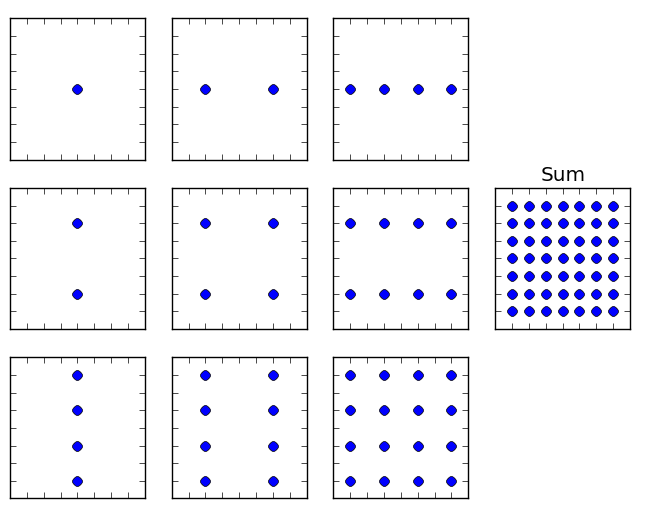
\includegraphics[width=7.5cm]{images/sparsegrid_hirach1}
      \vspace{-12px}
      \caption{}
    \end{figure}
  \end{block}
\end{frame}

\begin{frame}
  \frametitle{Sparse Grids -- Basics}
  \topline
  \vspace{-10px}
  \begin{block}{Hirachical subspaces}
    \begin{figure}[!htp]
      \setbeamertemplate{caption}{\raggedright\insertcaption\par}
      \setbeamerfont{caption}{size=\footnotesize}
      \centering
      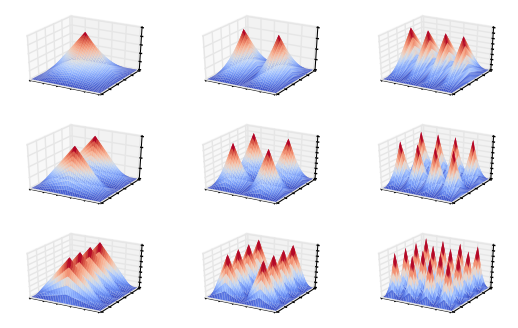
\includegraphics[width=7.5cm]{images/sparsegrid_2dhats}
      \vspace{-12px}
      \caption{}
    \end{figure}
  \end{block}
\end{frame}

\begin{frame}
  \frametitle{Sparse Grids -- Basics}
  \topline
  \vspace{-10px}
  \begin{block}{Sparse grid -- Changes}
    \begin{itemize}
      \item Throwing away certain subspaces
      \item Finding those is a \emph{a-priori} solvable optimization problem
      \item The resulting gird is now \textbf{sparse}
      \end{itemize}
  \end{block}
  \begin{block}{Profit}
    \begin{itemize}
      \item Reducing the computational effort ``a lot''
      \item Maintaining ``high'' accuracy
      \end{itemize}
  \end{block}
\end{frame}

\begin{frame}
  \frametitle{Sparse Grids -- Basics}
  \topline
  \vspace{-10px}
  \begin{block}{A \emph{sparse} grid}
    \begin{figure}[!htp]
      \setbeamertemplate{caption}{\raggedright\insertcaption\par}
      \setbeamerfont{caption}{size=\footnotesize}
      \centering
      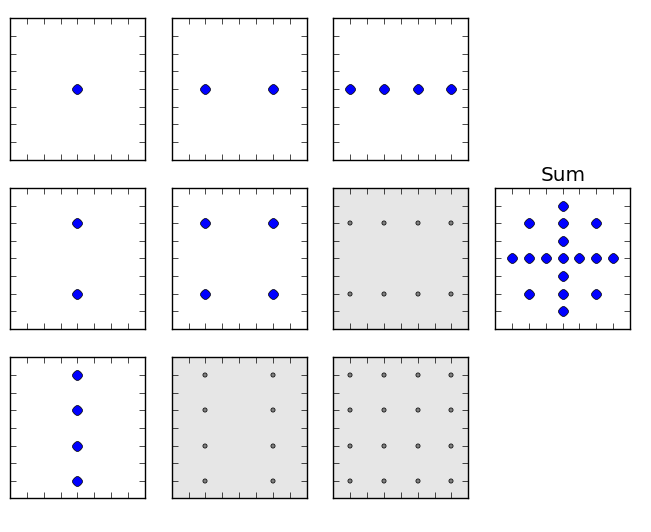
\includegraphics[width=7.5cm]{images/sparsegrid_hirach2}
      \vspace{-12px}
      \caption{}
    \end{figure}
  \end{block}
\end{frame}

\begin{frame}
  \frametitle{Sparse Grids -- Basics}
  \topline
  \vspace{-10px}
  \begin{block}{Boundry and smoothness}
    \begin{itemize}
      \item Boundries need special treatment
      \item The function needs to be sufficient smooth \\
        $D^2f$ needs to be bounded
      \end{itemize}
  \end{block}
  \begin{block}{Adaptivity}
    \begin{itemize}
      \item \emph{A-posteriori} modifications to better fit the function
      \item Picking a single gridpoint and adding level of detail around it
      \item Prone to overfitting and huge computational effort
      \end{itemize}
  \end{block}
\end{frame}


\begin{frame}
  \frametitle{Sparse Grids -- Basics}
  \topline
  \vspace{-10px}
  \begin{block}{Summary}
    \begin{itemize}
      \item Hirachial basis through grouping gridpoints into levels
      \item Creating ``subspaces'' through combination of levels in dimensions
      \item Selecting and combining subspaces
      \end{itemize}
  \end{block}
  \begin{block}{To keep in mind}
    \begin{itemize}
      \item Smoothness requirement for $f(x)$
      \item Boundry treatment
      \item Accuracy--effort trade-off
      \item Adaptivity options (\emph{a-posteriori})
      \end{itemize}
  \end{block}
\end{frame}



%%% Local Variables:
%%% TeX-master: "slides"
%%% End:

% Page 4
\section{Sparse Grids in Machine Learning}

As mentioned in the introduction, data mining scenarios with large datasets
and high-dimensional data are in general difficult to deal with.
Areas of application
that show these characteristics include engineering (e.g. heat-transfer
modeling) \cite{disspeh},
machine learning and data mining (e.g. estimation of cosmological redshifts
and option pricing in finance) \cite{disspfl}. In this section
we apply sparse grids to machine learning tasks
(classification and regression) relevant for data mining.
\par
\subsection{Least squares estimation}
A commonly used method in machine learning is \emph{least squares estimation}
$$\hat{c} = \underset{f}{\text{arg \hspace{-0.5mm}min}}\Bigg(\frac{1}{M}\sum\limits_{i = 1}^{M}{\Big(y^{(i)} - f(x^{(i)})\Big)^2 \ + \ \lambda R(f)} \Bigg)$$ \
using the notation for training data 
introduced in Sec.~\ref{sec:grid}. With this formula we
derive an estimator $\hat{c}$ that is the function which models the
data $X \times Y$ with the least error (minimization over $f$).
The term $R(f)$ is a regularization term to enforce smoothness. A common choice
is the $L_2$-Norm of the gradient of $f$: $R(f) = ||\nabla f||_2$.
\par
We will now use least squares estimation in a sparse grid setting. Intuitively,
$f$ and ultimately $\hat{c}$
 are functions discretized on a sparse grid and represented
accordingly:
$$\hat{c} = \underset{{\alpha}}{\text{arg \hspace{-0.5mm}min}}\Bigg(\frac{1}{M}
\sum\limits_{i = 1}^{M}{\Big(y^{(j)} - {\sum_{j=1}^N{\alpha_j}\phi_j(x^{(j)})}\Big)^2 +
  \lambda {\sum_{j=1}^N{\alpha_j^2}}}\color{black} \Bigg) \ .$$
Note, that for better readability the level-index $l$ is omitted here and
we now simply enumerate all grid points, basis functions $\phi_j$ and surpluses
$\alpha_j$
 by the index $j \in \{1..N\}$.
Also, the minimization now happens with
respect to the hierarchical surpluses $\alpha_j$,
which are the defining factor for $\hat{c}$.
When minimizing with respect to coefficients, $\sum_j^N{\alpha_j^2}$
is a common choice for
$R(f)$. Compared to the gradient, the
expressions in the following get simplified using this regularization
\cite{disspfl}.
\subsection{Matrix formulation}
Minimizing with respect to $\alpha$ leads to a system of linear equations that
can be formulated using the matrix expression
$$\Big(\frac{1}{M} BB^T + \lambda I \Big)\vec{\alpha} = \frac{1}{M}B\vec{y} \
.$$
The matrix
$$ \mathbb{R}^{N \times M} \ni B =
\begin{bmatrix}
  \phi_1(x^{(1)}) & \dots & \phi_1(x^{(M)}) \\
  \vdots & \ddots & \vdots \\
  \phi_N(x^{(1)}) & \dots  & \phi_N(x^{(M)}) \\
\end{bmatrix}
$$
sets the grid points in relation to the data points in $X$. By solving this
positive definite system we obtain the unique surplus-vector
$\vec{\alpha}$, defining $\hat{c}$ \cite{disshei}.
\par
The
matrix product $BB^T \in R^{N \times N}$ demonstrates that the number of freedoms
is not dependent on the number of data points. Thus, the computational effort
scales only linearly with respect to the number of data points $M$ \cite{disspfl}. Because
the matrix $B$ might have a lot of entries and is not sparse, methods like
Conjugate Gradients can be used to efficiently solve this system
of linear equations \cite{disshei}.

\subsection{Testing sparse grids}\label{subsec:test}
In order to get a good solution, several factors have to be determined before
sparse grids can be employed. The regularization parameter $\lambda$ and the
amount of refinement steps can be determined using cross-validation.
A straightforward way to refine grid points is to choose candidates
with high surplus $\alpha$. %as discussed in Sec.~\ref{subsec:ada}
For more
details on the choice of the refining strategy refer to \cite{disspfl}.
\par
First we examine the results of the checker-board dataset, a highly non-linear
classification test set (see Fig.~\ref{fig:fig4}).
While containing no noise, the checker-board-structured
distribution of points contains very steep areas, which are difficult to model.
Starting with a maximal level of $n=4$ (49 grid points)
the grid begins to capture the structure of the data with approximately
70\% correct classifications.
With a level of $n>7$ \ (796 grid points) more than 98\% are classified
correctly \cite{disspfl}. In both cases the grid was refined 8 times. For each
refinement-repetition the 5 grid points with the highest surplus $\alpha$ were chosen.
This demonstrates the ability of sparse grids
to model difficult non-linear datasets.
\par

\begin{figure*}[t!]
  \centering
  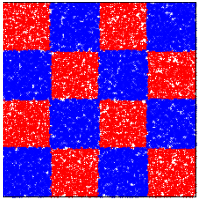
\includegraphics[width=0.3\textwidth]{images/figure_5_1.png}
  \hspace{10px}
  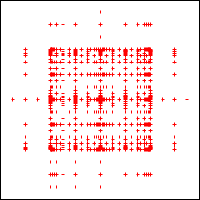
\includegraphics[width=0.3\textwidth]{images/figure_5_2.png}
  \hspace{10px}
  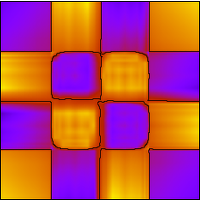
\includegraphics[width=0.3\textwidth]{images/figure_5_3.png}
  \captionsetup{width=0.95\textwidth}
  \caption{The checker-board test set. 40,000 sampled data points with
    $Y = \{-1, 1\}$ (colored red and blue respectively)
    used as training data (left).
    The refined sparse grid with 298 grid points (middle) and the
    projected decision manifold (right) showing high accuracy, especially
    towards the borders \cite{disspfl}.
    \label{fig:fig4}}
\end{figure*}


The second problem we examine is a real world regression
task.
A phenomenon similar to the doppler-effect called cosmological redshift
is modeled. The training data consists of photometric measurements from known
astronomical objects. By applying regression, the redshift of
newly observed objects is to be estimated using sparse grids.
The dataset available contains 60,000 data points with 5 dimensions. Even though
the shape of the data is inherently difficult to model, adaptive refinement
helps to capture the core features. In contrast to the previous
example, drastically more grid points are required to archive a low mean
squared error. At approximately 20,000 grid points the error drops
considerably. For a more detailed examination refer to \cite{disspfl}.
\par
These two examples demonstrate that sparse grids are able to cope with
non-linear, large and moderately high dimensional datasets. As previously
mentioned, spatial adaptivity is crucial to capture the features of the
problem and enables sparse grids to be a competitive method for data mining
and machine learning.

%\subsection{Further considerations}

%\begin{itemize}
%\item Quick note on classification/regression
%\item Least squares
%\item Least squarse with sparse grids
%\item Matrix formulation
%\item Notes on matrix solving etc.
%\end{itemize

%%% Local Variables:
%%% TeX-master: "report"
%%% End:


\end{document}